\documentclass[a4paper,11pt]{article}

\usepackage[english]{babel}
\usepackage{mathrsfs, amssymb, amsmath, amsthm, enumerate}
\usepackage{verbatim,graphicx,geometry}
%\usetikzlibrary{arrows}
\usepackage[utf8]{inputenc}
\usepackage{authblk}
\usepackage[round]{natbib}
\bibliographystyle{plainnat}

\usepackage{hyperref}

\makeatletter
\def\@biblabel#1{\hspace*{-\labelsep}}
\makeatother
\geometry{left=1in,right=1
in,top=1in,bottom=1in}
\newdimen\dummy
\dummy=\oddsidemargin
\addtolength{\dummy}{72pt}
\marginparwidth=.5\dummy
\marginparsep=.1\dummy


\newcommand{\E}{\mathbb{E}}
\newcommand{\Var}{\mathrm{Var}}
\newcommand{\plim}{\overset{p}{\longrightarrow}}
\newcommand{\dlim}{\overset{d}{\longrightarrow}}

\begin{document}

\begin{table}
\centering
\begin{tabular}{llll}
\hline \hline
variable & value & objective function & interpretation \\ \hline
$\eta^H$ & 0.06 & 1.0699 & New technology benefit \\
$\eta^M$ & 0.03 & 1.0699 & New combination benefit \\
$\tau$ & 200 & 1.0699 & Shape parameter for idea distribution \\
$\xi$ & 1 & 1.0699 & $1/\xi$ is the fraction of viable combinations \\
$\lambda $ & 1.5 & 1.0699 & scale parameter of the cost distribution \\
$\kappa $ & 0.2 & 1.0699 & shape parameter of the cost distribution \\
\hline \hline
\end{tabular}
\caption{Current values that minimize the objective function}
\end{table}


\begin{table}
\centering
\begin{tabular}{llll}
\hline \hline
Column \# & Moment & Model & Data \\ \hline
1 & Fraction of refinements in 1880 & 55.179\% & 55\% \\
2 & Fraction of new combinations in 1880 & 39.99\% & 30\% \\
3 & Fraction of new technologies in 1880 & 4.82\% & 10\% \\
4 & Fraction of refinements in 1930 & 29.054\% & 35\% \\
5 & Fraction of new combinations in 1930 & 68.09\% & 60\% \\
6 & Fraction of new technologies in 1930 & 2.84\% & 3\% \\
7 & Peak of the refinement share & 85.705\% & 60\% \\
8 & Year of the peak in refinement share & 1845 & 1870 \\
\hline \hline
\end{tabular}
\caption{Moments}
\end{table}


\begin{figure}
\begin{center}
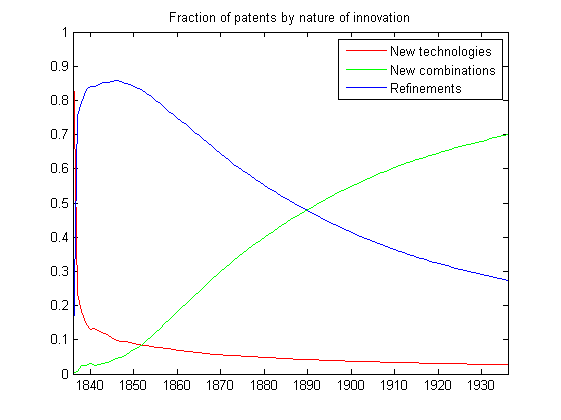
\includegraphics[scale=.8]{fractions.png}
\caption{Fraction of patents by type}
\end{center}
\end{figure}

\clearpage

\section*{Rate of growth of the economy}

There is a final good, produced with technology

\[ Y_t = \frac{L_t^{\gamma}}{1-\gamma}\sum_{j \in \mathcal{J}} q_{jt}^{\gamma}k_{jt}^{1-\gamma}. \]

Labor is inelastic, so $L_t \equiv 1$ and the profit maximization of firms implies $q_{jt} = k_{jt}$. This, in turn, gives

\[ Y_t = \frac{1}{1-\gamma}\sum_{j \in \mathcal{J}}q_{jt}. \]

Finally, we also have that the quality fo the product of a firm evolves according to

\[ q_{j,t+1} = q_{jt} + s_j\bar{q}_t \]
where $s_j$ is the quality of the patent that was purchased and $\bar{q}_t$ is the average quality in year $t$. 

Define the growth rate $g_t$ as

\[ g_t = \frac{Y_{t+1} - Y_t}{Y_t} = \frac{\frac{1}{1-\gamma}\sum_{j \in \mathcal{J}}q_{j,t+1} - \frac{1}{1-\gamma}\sum_{j \in \mathcal{J}}q_{jt}}{\frac{1}{1-\gamma}\sum_{j \in \mathcal{J}}q_{jt}} \]

Plugging in $q_{j, t+1}$, we have
\[ g_t = \frac{\sum_{j \in \mathcal{J}}s_j \bar{q}_t}{\sum_{j \in \mathcal{J}}q_{jt}} \]
and finally, using the definition of $\bar{q}_t$, we get

\[ g_t = \frac{\frac{1}{\mathcal{J}}\sum_{j \in \mathcal{J}}q_{jt}\sum_{j \in \mathcal{J}}s_j}{\sum_{j \in \mathcal{J}}q_{jt}} \]

\[ g_t = \frac{1}{\mathcal{J}}\sum_{j \in \mathcal{J}}s_j \]










\end{document}